\chapter{Pointers and memory allocation}

\section{Classifications of pointers}

Pointers are classified into two main categories:

\begin{itemize}
    \item \textbf{Raw pointers}: They are the most basic form of pointers, already present in \texttt{C} language. 
    They manually manage the memory allocation and deallocation.
    When using them, we have to be extremely careful to avoid memory leaks.
    \item \textbf{Smart pointers}: They are a part of the \texttt{C++11} standard, and are used to automate the memory management process.
    We wil come back to this later.
\end{itemize}

\section{Computer's memory}

The computer's memory is divided into four main sections:

\begin{itemize}
    \item \textbf{Code section}: It contains the program's executable code.
    \item \textbf{Static Data section}: It contains the global and static variables.
    \item \textbf{Heap section}: It is used for dynamic memory allocation. It is also called the \textit{free store}. It is
    managed by the \texttt{new} and \texttt{delete} operators.
    \item \textbf{Stack section}: It is used for local variables and function calls.
\end{itemize}

\begin{figure}[ht]
    \centering
    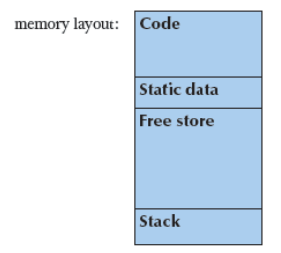
\includegraphics[width=4.5cm]{figures/image_memory.png}
    \caption{Memory layout}
    \label{fig:memory}
\end{figure}

\subsection{Heap section (free store)}

You request memory to be allocated in the heap using the \texttt{new} operator. This operator returns a pointer to the allocated memory,
which is just the address of the first byte of that memory block. For example:\\

\begin{lstlisting}[language=C++]
int *p = new int; // allocate one uninitialized integer
int *q = new int[10]; // allocate an array of 10 uninitialized integers
double *r = new double[4]; // allocate an array of 4 uninitialized doubles
\end{lstlisting}

A pointer points to an object of its specific type, but it does not know how many elements it points to.\\

To deallocate memory in the heap, you use the \texttt{delete} operator. For example:\\

\begin{lstlisting}[language=C++]
delete p; // deallocate the memory pointed by p
delete[] q; // deallocate the memory pointed by q
delete[] r; // deallocate the memory pointed by r
\end{lstlisting}

\section{Pointer states}

The value (i.e., the address) stored in a pointer can be in one of the following four states:

\begin{enumerate}
    \item It can point to an object.
    \item It can point to the location just past the end of an object.
    \item It can be a null pointer, indicating that it does not point to any object.
    \item It can be an invalid pointer; that is, values that are not any of the above.
\end{enumerate}

It is an error to copy or try to access the value of an invalid pointer. As when we use an uninitialized pointer,
this error is one that the compiler is unlikely to detect. The result of using an invalid pointer is undefined, so
we must always ensure that a pointer is valid before using it.\\

\subsection{Null pointers}

A null pointer is a pointer that does not point to any object. It is represented by the literal \texttt{nullptr}.
The code can check if a pointer is null by comparing it to \texttt{nullptr}. For example:\\

\begin{lstlisting}[language=C++]
int *p = nullptr; // p is a null pointer
if (p == nullptr) {
    std::cout << "p is a null pointer" << std::endl;
}
\end{lstlisting}

The \texttt{nullptr} is a keyword that represents a null pointer. It is a pointer literal that can be converted to any pointer type.
Be aware that a better practice is to rely on short-circuit evaluation to check if a pointer is null. For example:\\

\begin{lstlisting}[language=C++]
// some code...
if (p != nullptr && *p == 10) {
    std::cout << "p is not null and points to 10" << std::endl;
}
// some more code...
\end{lstlisting}

\section{Pointer arithmetic and array access}

We can perform arithmetic operations on pointers. For example, we can increment or decrement a pointer, or add or subtract an integer
from a pointer. When doing so, the compiler automatically scales the integer by the size of the type the pointer points to. This is the 
way that arrays are accessed in \texttt{C++}. For example:\\

\begin{lstlisting}[language=C++]
int arr[5] = new int[5];
int *p = arr; // p points to the first element of arr
std::cout << *p << std::endl; // prints 1
p++; // p now points to the second element of arr
std::cout << *p << std::endl; // prints 2
\end{lstlisting}

Note that when we try to access a specific element of an array, we can use the subscript operator \texttt{[]}. For example:\\

\begin{lstlisting}[language=C++]
int arr[5] = new int[5];
std::cout << arr[0] << std::endl; // prints 1
std::cout << arr[1] << std::endl; // prints 2
\end{lstlisting}

This is equivalent to the following code:\\

\begin{lstlisting}[language=C++]
int arr[5] = new int[5];
int *p = arr; // p points to the first element of arr
std::cout << *p << std::endl; // prints 1
std::cout << *(p + 1) << std::endl; // prints 2
\end{lstlisting}

We have to be careful, as the pointer itself does not know how many elements it points to. So, although it is valid to
subscript a negative index, or an out of bounds index (since it is just an arithmetic operation), it is not safe to do so, and
it leads to undefined behavior and undetectable errors. Let us see an example:\\

\begin{lstlisting}[language=C++]
int arr[5] = new int[5];
arr[-1] = 10; // undetected error
arr[5] = 10; // undetected error
\end{lstlisting}

Note that \texttt{arr[-1]} is equivalent to \texttt{*(arr - 1)}, and \texttt{arr[5]} is equivalent to \texttt{*(arr + 5)}, but
they both are pointers to memory that has not been allocated for the array \texttt{arr}.\\

A pointer does know the size of the type it points to, and that is why we can use pointer arithmetic to access the elements of an array.
Unlike other types (e.g. \texttt{int} and \texttt{double}), there is no implicit conversion between pointers to different types.

\section{Why use pointers and free store?}

With the \texttt{C} language, we use the heap memory when we don't know a priori the size of the data structure and 
we don't want to waste memory. For example, when we want to create a linked list, we don't know how many elements
it will have, so we use the heap memory to allocate memory for each element.\\

Note that with pointers and arrays, we are "touching" the hardware directly, so we have to be careful when using them.
Here is where serious programming errors can most easily occur, resulting in malfuntioning programs, or even worse,
programs that appear to work correctly but are subtly incorrect (obscure bugs). If we get "segmentation fault",
"bus error", or "core dumped", it is likely that we are using pointers incorrectly.\\

In \texttt{C++}, we have the STL containers, like \texttt{std::vector}, which automatically manage 
the memory for us. We will come back to this later.\\

We mainly use free store to allocate objects that have to outlive the scope in which they are created. For example, when we
want to return a pointer to an object from a function, we have to allocate memory in the heap, as the stack memory is deallocated
when the function returns. This is an example of this case:\\

\begin{lstlisting}[language=C++]
// some code...
double *create_array(int n) {
    double *arr = new double[n];
    return arr;
}
// some more code...
\end{lstlisting}

We mainly use raw pointers when we want to share large data structures and avoid multiple copies of them. Note that copies not only waste
memory, but also need to be kept in sync, introducing additional overhead.

\section{Memory leaks}

A memory leak occurs when a program allocates memory in the heap and does not deallocate it. This memory is not available for
other programs, and it is lost. This is a serious problem, as it can lead to the exhaustion of the available memory, and the program
can crash.\\

Let us see an example:

\begin{lstlisting}[language=C++]
double *calc(int result_size, int max){
    int *p = new double[max];
    double *result = new double[result_size];
    // use p to calculate results to be put in result...
    return result;
}

int main(){
    double *res = calc(10, 100); // we forgot to deallocate p
    return 0; // we forgot to deallocate res
}
\end{lstlisting}

In this case, we have a memory leak, as we forgot to deallocate the memory pointed by \texttt{p}. To avoid memory leaks, we have to
always deallocate the memory we allocate in the heap, by using the \texttt{delete} operator. Here is the fixed code:\\

\begin{lstlisting}
double *calc(int result_size, int max){
    int *p = new double[max];
    double *result = new double[result_size];
    // use p to calculate results to be put in result...
    delete[] p; // deallocate p
    return result;
}

int main(){
    double *res = calc(10, 100);
    delete[] res; // deallocate res (this is easy to forget)
    return 0;
}
\end{lstlisting}

A program that needs to run for a long time can't afford any memory leaks, as they accumulate over time. An example of
this is an operating system, which has to run for a long time without crashing.\\

Nonetheless, programs that run to completion with predictable memory usage may leak without causing problems, i.e., memory
leaks aren't "good/bad", but they can be a major problem in specific circumstances.\\

Another way of getting memory leaks is when we overwrite the pointer to the allocated memory before deallocating it. For example:\\

\begin{lstlisting}[language=C++]
double *p = new double[10];
p = new double[20]; // we lost the pointer to the first memory block
delete[] p; // we deallocate the memory pointed by p, but it is not the memory we allocated
\end{lstlisting}

In this case, we have a memory leak, as we lost the pointer to the first memory block. To avoid this, we have to always deallocate
the memory before overwriting the pointer.\\

\subsection{How to avoid memory leaks}

To systematically avoid memory leaks, we can follow these rules:

\begin{itemize}
    \item Don't mess directly with \texttt{new} and \texttt{delete}, unless you have to. Try to use the STL containers.
    \item Use a garbage collector. This is a program that keeps track of all the memory you allocated dynamically.
    \item In \texttt{C++}, use smart pointers. They are a part of the \texttt{C++11} standard, and are used to automate 
    the memory management process (more on this later).
\end{itemize}

Unfortunately, not even garbage collectors or smart pointers can prevent all memory leaks.

\section{Free store summary}

\begin{itemize}
    \item Allocate using \texttt{new}:\\
    \texttt{new} allocates an object on the free store, sometimes initializes it, and returns a pointer to it.

    \begin{lstlisting}[language=C++]
        int *p = new int; // allocate one uninitialized integer
        char *q = new char('a'); // allocate one initialized char
        double *r = new double[10]; // allocate an array of 10 uninitialized doubles
    \end{lstlisting}

    \item Deallocate using \texttt{delete} and \texttt{delete[]}:\\
    \texttt{delete} deallocates an object on the free store, and \texttt{delete[]} deallocates an array of objects on the free store.

    \begin{lstlisting}[language=C++]
        delete p; // deallocate p
        delete q; // deallocate q
        delete[] r; // deallocate array r
    \end{lstlisting}

    \item Delete of null pointers does nothing:
    \begin{lstlisting}[language=C++]
        int *p = nullptr;
        delete p; // harmless
    \end{lstlisting}

\end{itemize}